\documentclass[conference]{IEEEtran}
\IEEEoverridecommandlockouts
\usepackage{cite}
\usepackage{amsmath,amssymb}
\usepackage{fontspec}
\setmainfont{texgyretermes}[Extension=.otf, UprightFont=*-regular, BoldFont=*-bold,
  ItalicFont=*-italic, BoldItalicFont=*-bolditalic]
\setmonofont{texgyrecursor}[Extension=.otf, UprightFont=*-regular, BoldFont=*-bold,
  ItalicFont=*-italic, BoldItalicFont=*-bolditalic]
\usepackage{graphicx}
\usepackage{booktabs}
\usepackage{array}
\usepackage{url}
\usepackage{tikz}
\usetikzlibrary{positioning,arrows.meta,fit,backgrounds,calc}
\renewcommand{\arraystretch}{1.1}
\def\UrlBreaks{\do\/\do-\do.\do\#}

\begin{document}

\title{Privacy-Preserving Context-Aware Password Risk Assessment with Cross-Account Dependency Analysis and Save-Time Intervention}

\author{\IEEEauthorblockN{Jasmeet Ranjan Srivastava, Garvit Singla, Rakshit Kapoor}
\IEEEauthorblockA{Department of Computer Science and Engineering (Information Security)\\
Vellore Institute of Technology, Vellore, Tamil Nadu, India}}

\maketitle

\begin{abstract}
A password can be structurally strong yet predictable from its owner's personal details or other passwords. We present the Context-Aware Local Vault (CAV), a local-first password manager. It combines k-anonymity breach checks, coverage of personal attributes the user declares, zxcvbn structural weakness, reuse and derivative-password families. It encrypts credentials and the personal profile, and it can warn before a risky password is stored. Under protocols frozen before each analysis, we test whether these signals detect attack-recoverable passwords. On a synthetic fixture of 11,022 examples, the fixed-weight risk score's recall against an all-information attacker was 0.153 at a 5\% false-positive limit, equal to breach evidence alone. Without breach evidence the score cannot exceed 0.50, below its 0.60 threshold. On an independent benchmark of 1,000 real users' breached passwords (PASS), a history attacker recovered 48.9\% of target passwords from each user's other passwords. CAV's cross-account rule detected 99.8\% of these recoveries at a 14.3\% false-positive rate, compared with 97.5\% at 47.9\% for zxcvbn given the same history. On targets that were not exact reuse, the rule's recall was 17.2 points higher and its false-positive rate 33.7 points lower. The fixed score flagged none of these passwords, and logistic models fitted on synthetic data did not transfer. The personal-context detector, which this benchmark cannot test, missed unseen transformations and accent-free or transliterated names. The vault adds authenticated backups, per-device Argon2id calibration and concealed clipboard copies, and 157 tests pass. A hosted four-condition intervention study is ready but has not been run.
\end{abstract}

\begin{IEEEkeywords}
Password management, personal context, targeted password guessing, derivative passwords, k-anonymity, envelope encryption, save-time intervention.
\end{IEEEkeywords}

\section{Introduction}
Passwords remain a common way to prove identity online, and password managers and two-factor tools are the usual response to their weaknesses~\cite{jubur}. Two problems persist. First, people reuse passwords across work and personal accounts~\cite{aiswarya}, so one exposed credential can open several services~\cite{farcasin}. Second, people build passwords from things they know about themselves, such as names, hometowns and birth years. These details are often easy to find in public profiles~\cite{atzori2024}. Composition rules do not reliably improve resistance to cracking~\cite{he}, and rigid policies increase the burden on users, who respond with insecure coping strategies~\cite{umejiaku2023}. AI-assisted, multi-component assessment has precedent in other security domains~\cite{nebbione}. Targeted attacks that combine personal information with a user's old passwords are well established~\cite{ou2026,mdiguess}.

Existing meters address part of this problem. zxcvbn estimates guessing effort from patterns, dictionary terms and keyboard walks~\cite{wheeler}, but it does not check whether a password appears in breach data or whether it is built from the owner's personal details. Saint-Jean et al. reported that structural strength and breach exposure are nearly uncorrelated and proposed combining them~\cite{saintjean}. Personal-context assessment~\cite{atzori2024,alatawi} and multi-source targeted guessing~\cite{mdiguess} already exist, so integrating them is not novel in itself. The question we examine is narrower: whether a local assessment that also uses relationships between the credentials in one vault adds measurable detection value, and whether acting before a password is stored can be studied in a controlled way.

We address four research questions. \textbf{RQ1:} Does locally declared personal context improve attack-relevant detection relative to conventional strength estimation at a controlled false-positive rate? \textbf{RQ2:} Do cross-account relationships improve detection under history-aware attackers, and what does transitive clustering cost? \textbf{RQ3:} Does pre-save feedback reduce vulnerable retained credentials relative to equivalent post-save feedback, and does an immediate alternative add benefit? \textbf{RQ4:} Can these behaviours be delivered with acceptable local privacy exposure and computational overhead? This paper answers RQ1, RQ2 and RQ4 on synthetic data only, and specifies RQ3 without running it. It is therefore an evaluation paper. The fixed-weight score's weak operational performance is reported as the central finding, and no superior detection is claimed.

The contributions are as follows.
\begin{enumerate}
\item A controlled evaluation, under a protocol frozen before the experiments, of a contextual heuristic score. It compares the score against matched baselines, fixed non-additive rules, and unconstrained and non-negative logistic models, with profile-level confidence intervals. The evaluation identifies a threshold failure mode: an additive score whose contextual terms are capped below its operating threshold cannot flag risk that comes only from personal context or password history.
\item An analysis of bias in synthetic evaluation. It covers field attribution for stress-test transformations, fixture artefacts that cause false alarms, and attacker-stream exhaustion, which makes budgets above 1,000 guesses uninformative for this attacker.
\item A local vault implementation that keeps the signals separate, reports unknown breach status as an interval, and encrypts credentials and the personal profile. It adds authenticated backups, per-device Argon2id calibration and an exact indexed derivative search. These are established mechanisms, not a new cryptographic contribution.
\item An independent real-data evaluation of the cross-account signals on the public PASS benchmark of breached passwords~\cite{pass}. Thresholds and models were frozen from the synthetic validation, and the comparison is paired against a published contextual meter.
\item An instrument for studying intervention timing, with concealed block randomization, counterbalanced tasks, the System Usability Scale and a sample-size simulation. No behavioural efficacy is claimed.
\end{enumerate}

\section{Related Work}
\textbf{Strength estimation and breach exposure.} Early composition policies counted character classes. Modern meters estimate guessing effort from patterns~\cite{wheeler}. Probabilistic context-free grammars model password structure from breach corpora, and PCFG-based cracking was formalized by Weir et al.~\cite{weir}. Breach exposure is a separate dimension. Saint-Jean et al. proposed $E_{\text{final}}=\min(E_{\text{base}},E_{\text{breach}})$ to capture high-entropy breached passwords~\cite{saintjean}. NIST guidance favours length and blocklist screening over composition rules and periodic changes~\cite{nist63b4}. CAV follows that direction but keeps breach status, structure and personal context as separate signals rather than collapsing them into a single minimum.

\textbf{Neural and data-driven guessing.} Recurrent models have been applied to password and passphrase guessing~\cite{nosenko}. Sun~\cite{sun} proposed a hybrid ResCNN-BiGRU-GAP model that classifies the origin of a password, reporting an F1-macro of 0.952 on that task. Xu et al.~\cite{xu} showed that client-side strength meters built from data-driven models can leak training data through membership inference. This motivates keeping strength evaluation on the device and avoiding distribution of trained models. CAV's live checks are rule-based and lookup-based. The logistic models in Section~\ref{sec:results} are research baselines. No application page loads a fitted model (Section~\ref{sec:assess}).

\textbf{Personal context and targeted guessing.} SODA ADVANCE reconstructs biographical profiles from social networks and scores passwords against them using CUPP-style dictionaries, leetspeak decoding and coverage metrics~\cite{atzori2024,atzori2025}. G\"uven et al.~\cite{guven} showed that users with multiple breached accounts follow predictable mutation patterns. Wang et al.~\cite{pass} analysed 61.5 million passwords of 28.8 million users across 107 services and released a public sample, which we use as an independent benchmark. Ou et al.~\cite{ou2026} combined personally identifiable information with old passwords for targeted guessing, and MDIGuess~\cite{mdiguess} jointly exploits historical passwords, personal information and general leaked-password data. Cipher-Guard~\cite{alatawi} adds context to a machine-learning password assessment. CAV keeps the coverage and leetspeak ideas but replaces scraping with fields that the user declares, so no third-party profile data is collected. Our bounded attacker is a simple deterministic generator. It is not a reproduction of these attacks, and their reported metrics are not comparable with ours.

\textbf{Language models and passwords.} Honeyword systems place decoy passwords beside real ones to detect database theft, and deep learning has been used to separate honeywords from real passwords~\cite{dani}. LLM-based honeyword generation~\cite{umejiaku2025} and LLM password generation~\cite{kagnici} show both defensive uses and predictability risks, and LLMs can also support targeted social engineering~\cite{sai}. An earlier CAV design asked a hosted model for passphrases. Its output did not reliably meet the prompt's constraints, and model output provides no verifiable generation entropy. The current build therefore generates all suggestions locally.

\textbf{Nudging and intervention timing.} A PRISMA-based review of cybersecurity nudges identified informational, default, framing and social nudges, and it reported that feedback and effort-reduction designs produced the most durable effects~\cite{arciulo}. Protection Motivation Theory separates threat appraisal from coping appraisal. Zou et al. found that threat messages alone did not change password behaviour, whereas pairing threat messages with coping advice did~\cite{zou}. Personalized nudges have improved compliance in some settings~\cite{peer}, and lyric-based passphrases can be easier to recall~\cite{wise}. Rather than inferring effectiveness from suggestion acceptance, CAV's study interface is designed to compare intervention timing and the presence of an alternative directly. It has not yet been run with participants.

Table~\ref{tab:capabilities} summarizes the capabilities stated in the cited descriptions of these works. It compares inputs and settings, not accuracy: the works use different data, attackers and outcomes, so their reported metrics are not comparable with ours.

\begin{table}[t]
\caption{Capabilities Stated in the Cited Work}
\label{tab:capabilities}
\centering\scriptsize
\setlength{\tabcolsep}{2.6pt}
\begin{tabular}{@{}l l c c c c c c c@{}}
\toprule
Work & Role & Str. & Br. & Pers. & Hist. & Local & Pre-save & Users\\
\midrule
zxcvbn~\cite{wheeler} & meter & \checkmark & -- & -- & -- & \checkmark & -- & --\\
Saint-Jean~\cite{saintjean} & model & \checkmark & \checkmark & -- & -- & -- & -- & --\\
SODA ADV.~\cite{atzori2024} & meter & -- & -- & \checkmark$^{a}$ & -- & -- & -- & --\\
Ou et al.~\cite{ou2026} & attack & -- & -- & \checkmark & \checkmark & -- & -- & --\\
MDIGuess~\cite{mdiguess} & attack, meter & \checkmark$^{b}$ & -- & \checkmark & \checkmark & -- & -- & --\\
Zou et al.~\cite{zou} & intervention & -- & \checkmark & -- & -- & -- & -- & \checkmark\\
CAV (this work) & vault, meter & \checkmark & \checkmark & \checkmark$^{c}$ & \checkmark$^{d}$ & \checkmark & \checkmark & --$^{e}$\\
\bottomrule
\multicolumn{9}{@{}p{\columnwidth}@{}}{\scriptsize Str.: structural strength; Br.: breach exposure; Pers.: personal information; Hist.: old or other passwords; Local: assessment on the user's device; Users: human-subject evaluation. \checkmark: stated in the cited description; --: not stated. $^{a}$Profiles reconstructed from social networks. $^{b}$General leaked-password data. $^{c}$Declared by the user, not scraped. $^{d}$Other passwords in the same vault. $^{e}$Study interface built; no participants yet.}
\end{tabular}
\end{table}

\section{Threat Model and Design Goals}
\label{sec:threat}
\textbf{Adversaries.} Table~\ref{tab:threats} lists the five adversaries, the access each is assumed to have, where each is evaluated and what remains outside the evidence. The attacker in A3 is the deterministic generator described in Section~\ref{sec:method}. Its knowledge levels S1--S5 range from general statistics only (S1), through personal identifiers (S2) and one prior password (S3), to both together (S4) and all three sources (S5).

\begin{table}[t]
\caption{Adversaries, Assumed Access and Evidence}
\label{tab:threats}
\centering\scriptsize
\begin{tabular}{@{}p{1.0cm}p{2.3cm}p{1.9cm}p{2.2cm}@{}}
\toprule
Adversary & Access and assumptions & Evaluated by & Not covered\\
\midrule
A1 locked storage & Reads or edits the database or backup files; no key and no unlocked session & Tamper, manifest, rollback and deletion tests (Table~\ref{tab:sec}) & Whole-vault rollback; live row deletion; visible lengths and counts\\
A2 online guessing & Uses the app's unlock and recovery screens repeatedly & Throttling tests; Argon2id timing & Offline guessing cost on attacker hardware\\
A3 targeted guessing & Offline; knows S1--S5 information; up to $10^5$ guesses & E2, E3 & Published neural attacks; real users\\
A4 network observer & Sees breach-check traffic & Application-layer and packet capture & Timing and frequency of checks; one network\\
A5 environment & Clipboard contents; session state after lock & Real macOS pasteboard; session tests & OS or third-party clipboard history; immutable Python copies\\
\bottomrule
\end{tabular}
\end{table}

\textbf{Out of scope.} Malware controlling an unlocked session, a compromised browser or operating system, forensic recovery of historical snapshots or old file copies, malicious dependencies, multi-device synchronization, browser autofill and enterprise single sign-on are outside the guarantees. Rollback or deletion of a whole previously valid vault is not prevented; Section~\ref{sec:results} tests and reports this.

\textbf{Design goals.} (D1) No plaintext credentials or personal-profile fields in protected storage. (D2) Passwords and personal attributes never leave the device. (D3) Warnings reflect separate signals, and missing evidence is reported as missing rather than as safe. (D4) Intervention can occur before a credential is committed, with a usable alternative at the same moment.

\section{System Architecture}
CAV is a Python application built with Streamlit and bound to the loopback address 127.0.0.1, with usage statistics disabled. Its pages are My Vault, Security Audit, Password Generator, Import and Backup, Settings and Profile, a Legacy Advisor Pilot, and a Controlled Study page for conditions G1--G4. The vault pages share one authentication gate. The study page never accesses the real vault. Fig.~\ref{fig:arch} shows the components and data flows.

\begin{figure*}[t]
\centering
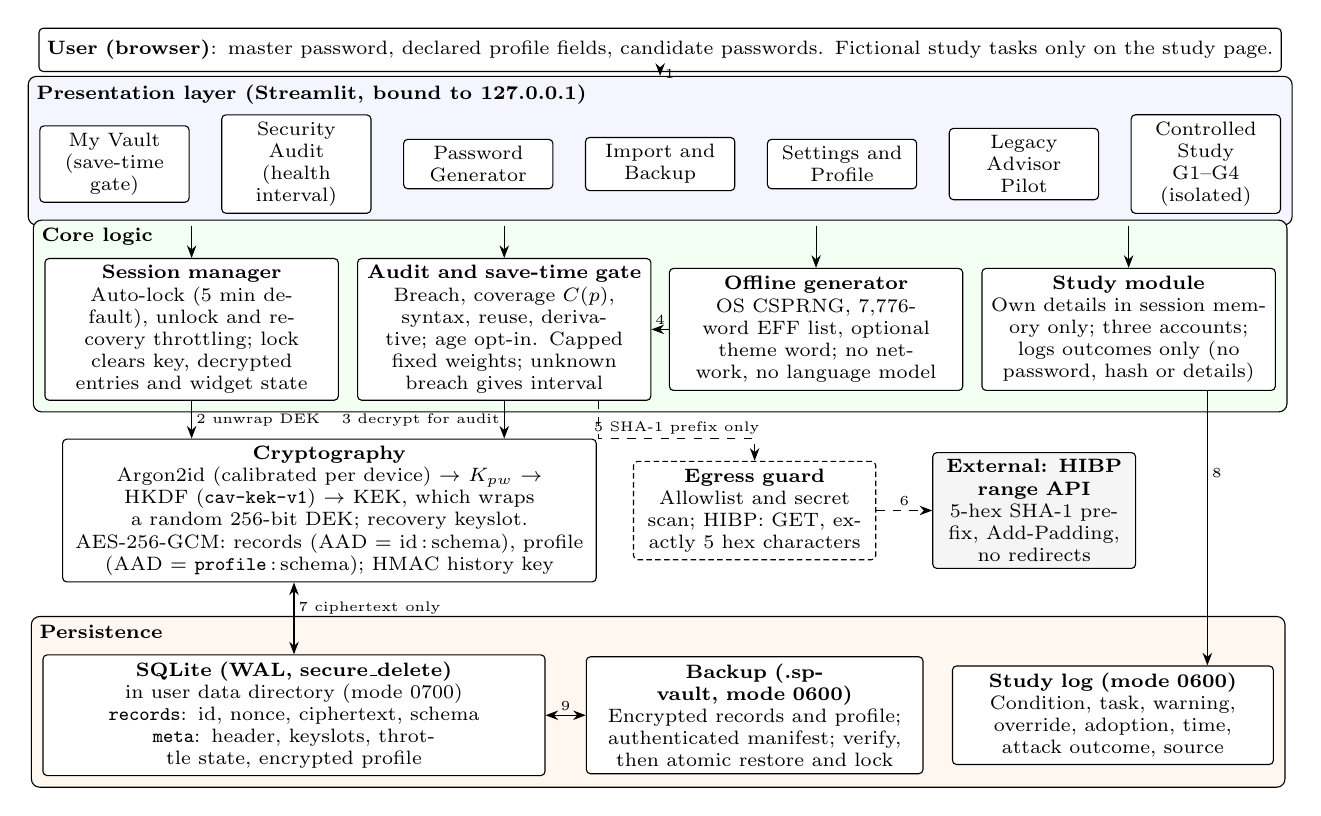
\begin{tikzpicture}[
  font=\scriptsize,
  >={Stealth[length=1.6mm]},
  box/.style={draw, rounded corners=1.5pt, align=center, inner sep=2.5pt, fill=white},
  page/.style={box, text width=1.72cm, minimum height=0.62cm},
  core/.style={box, text width=3.55cm, minimum height=1.55cm},
  layer/.style={draw, rounded corners=3pt, inner sep=4pt},
  lab/.style={font=\scriptsize\bfseries, anchor=north west, inner sep=3pt},
  num/.style={font=\tiny, inner sep=1.5pt}
]
% User
\node[box, text width=15.6cm, minimum height=0.55cm] (user) at (0,0)
  {\textbf{User (browser)}: master password, declared profile fields, candidate passwords. Fictional study tasks only on the study page.};
% Pages
\begin{scope}[yshift=-1.45cm]
\node[page] (p1) at (-6.93,0) {My Vault\\(save-time gate)};
\node[page] (p2) at (-4.62,0) {Security Audit\\(health interval)};
\node[page] (p3) at (-2.31,0) {Password\\Generator};
\node[page] (p4) at (0,0) {Import and\\Backup};
\node[page] (p5) at (2.31,0) {Settings and\\Profile};
\node[page] (p6) at (4.62,0) {Legacy Advisor\\Pilot};
\node[page] (p7) at (6.93,0) {Controlled Study\\G1--G4 (isolated)};
\end{scope}
% Core
\begin{scope}[yshift=-3.55cm]
\node[core] (sess) at (-5.95,0) {\textbf{Session manager}\\Auto-lock (5 min default), unlock and recovery throttling; lock clears key, decrypted entries and widget state};
\node[core] (aud) at (-1.98,0) {\textbf{Audit and save-time gate}\\Breach, coverage $C(p)$, syntax, reuse, derivative; age opt-in. Capped fixed weights; unknown breach gives interval};
\node[core] (gen) at (1.98,0) {\textbf{Offline generator}\\OS CSPRNG, 7,776-word EFF list, optional theme word; no network, no language model};
\node[core] (stu) at (5.95,0) {\textbf{Study module}\\Own details in session memory only; three accounts; logs outcomes only (no password, hash or details)};
\end{scope}
% Crypto, egress and external service
\begin{scope}[yshift=-5.85cm]
\node[box, text width=6.6cm, minimum height=1.25cm] (cry) at (-4.2,0) {\textbf{Cryptography}\\Argon2id (calibrated per device) $\rightarrow$ $K_{pw}$ $\rightarrow$ HKDF (\texttt{cav-kek-v1}) $\rightarrow$ KEK, which wraps a random 256-bit DEK; recovery keyslot.\\AES-256-GCM: records (AAD = id\,:\,schema), profile (AAD = \texttt{profile}\,:\,schema); HMAC history key};
\node[box, text width=2.9cm, minimum height=1.25cm, dash pattern=on 2pt off 1.2pt] (egr) at (1.2,0) {\textbf{Egress guard}\\Allowlist and secret scan; HIBP: GET, exactly 5 hex characters};
\node[box, text width=2.4cm, minimum height=1.25cm, fill=gray!8] (hibp) at (4.75,0) {\textbf{External: HIBP range API}\\5-hex SHA-1 prefix, Add-Padding, no redirects};
\end{scope}
% Persistence
\begin{scope}[yshift=-8.45cm]
\node[box, text width=6.2cm, minimum height=1.15cm] (db) at (-4.65,0) {\textbf{SQLite (WAL, secure\_delete)} in user data directory (mode 0700)\\\texttt{records}: id, nonce, ciphertext, schema\\\texttt{meta}: header, keyslots, throttle state, encrypted profile};
\node[box, text width=4.1cm, minimum height=1.15cm] (bak) at (1.2,0) {\textbf{Backup (.spvault, mode 0600)}\\Encrypted records and profile; authenticated manifest; verify, then atomic restore and lock};
\node[box, text width=3.9cm, minimum height=1.15cm] (log) at (5.75,0) {\textbf{Study log (mode 0600)}\\Condition, task, warning, override, adoption, time, attack outcome, source};
\end{scope}
% Layer frames with a title strip above the boxes
\coordinate (presTop) at ($(p7.north)+(0,0.34)$);
\coordinate (coreTop) at ($(sess.north)+(0,0.34)$);
\coordinate (persTop) at ($(db.north)+(0,0.34)$);
\begin{scope}[on background layer]
\node[layer, fill=blue!4, fit=(p1)(p7)(presTop)] (pres) {};
\node[layer, fill=green!5, fit=(sess)(stu)(coreTop)] (corel) {};
\node[layer, fill=orange!6, fit=(db)(log)(persTop)] (pers) {};
\end{scope}
\node[lab] at (pres.north west) {Presentation layer (Streamlit, bound to 127.0.0.1)};
\node[lab] at (corel.north west) {Core logic};
\node[lab] at (pers.north west) {Persistence};
% Flows
\draw[->] (user.south) -- node[num, right]{1} (pres.north);
\draw[->] (sess.north |- pres.south) -- (sess.north);
\draw[->] (aud.north |- pres.south) -- (aud.north);
\draw[->] (gen.north |- pres.south) -- (gen.north);
\draw[->] (stu.north |- pres.south) -- (stu.north);
\draw[->] (sess.south) -- node[num, right]{2 unwrap DEK} (sess.south |- cry.north);
\draw[->] (aud.south) -- node[num, left]{3 decrypt for audit} (aud.south |- cry.north);
\draw[->] (gen.west) -- node[num, above]{4} (aud.east);
\draw[->, dashed] ($(aud.south)+(1.2,0)$) -- ++(0,-0.48) -| node[num, pos=0.25, above]{5 SHA-1 prefix only} (egr.north);
\draw[->, dashed] (egr.east) -- node[num, above]{6} (hibp.west);
\draw[<->] (cry.south -| db.north) -- node[num, right, pos=0.35]{7 ciphertext only} (db.north);
\coordinate (s8) at ($(stu.south)+(1.0,0)$);
\draw[->] (s8) -- node[num, right, pos=0.3]{8} (s8 |- log.north);
\draw[<->] (db.east) -- node[num, above]{9} (bak.west);
\end{tikzpicture}
\caption{CAV architecture. Solid arrows are local data flows and dashed arrows are network flows. The only external destination is the HIBP range endpoint. Numbered flows: (1) user input, (2) key unwrap at unlock, (3) decryption for audit, (4) replacement passphrase, (5, 6) breach range query, (7) ciphertext storage, (8) study outcome logging and (9) backup and restore. Credentials and the personal profile are stored only as ciphertext. The study page keeps participants' details and passwords in session memory only and never writes to the vault.}
\label{fig:arch}
\end{figure*}

The system is organized in six layers. The \emph{presentation} layer contains the Streamlit pages and shared helpers, and every vault page checks for an unlocked session. The \emph{session} layer handles auto-lock, unlock throttling and in-memory key handling. The \emph{audit and gate} layer analyses decrypted entries in memory and checks candidate credentials at save time. The \emph{cryptography} layer performs key derivation, key wrapping and record and profile encryption. The \emph{persistence} layer uses SQLite in WAL mode with secure deletion enabled. The \emph{network boundary} is an egress guard that inspects outbound requests.

\section{Cryptographic Design}
\textbf{Key hierarchy.} The master password is processed by Argon2id~\cite{rfc9106}, producing a 32-byte password key $K_{pw}$. Parameters are chosen once, when a vault is created, and stored in its header. The calibration uses 256\,MiB of memory and 4 lanes and picks the iteration count from a measured per-iteration time. It then increases the count until one derivation takes at least 300\,ms on the creating device, never going below RFC 9106's second recommended setting of 64\,MiB, $t=3$ and $p=4$. Existing vaults keep their stored parameters. A key-encryption key (KEK) is derived from $K_{pw}$, optionally combined with a device secret, using HKDF-SHA256~\cite{rfc5869} with the context label \texttt{cav-kek-v1}. A random 256-bit data-encryption key (DEK) encrypts every record. The DEK is wrapped under the KEK with AES-256-GCM~\cite{gcm} to form a password keyslot. A separate 256-bit recovery key, shown to the user once in grouped base32 form, wraps the DEK in a recovery keyslot. A history key derived from the DEK with the label \texttt{cav-hist-hmac-v1} produces HMAC-SHA256 digests of previous passwords, so reuse can be detected without storing plaintext history. Changing the master password re-wraps the DEK; records are not re-encrypted.

\textbf{Associated data.} Keyslot wraps are authenticated over the canonical header, excluding the keyslot ciphertexts to avoid circular dependence. Each record is authenticated with its identifier and schema version, so ciphertext cannot be moved between rows without detection.

\textbf{Record and profile encryption.} An entry is serialized as canonical JSON with sorted keys and encrypted with AES-256-GCM under the DEK, using a fresh 96-bit nonce. The records table stores only the identifier, nonce, ciphertext with tag and schema version. The personal profile (first name, surname, city, birth year and theme) is encrypted under the same DEK and bound to the label \texttt{profile} and the schema version. Writing a profile without an unlocked DEK raises an authentication error, so there is no plaintext write path. A legacy plaintext profile is not returned while the vault is locked. It is migrated to ciphertext on the first authenticated read, and a failed migration is reported rather than suppressed. SQLite secure deletion is enabled for future deletions and updates. It does not erase historical copies, snapshots or flash-storage remnants.

\textbf{Backup and restore.} Encrypted backups use a \texttt{.spvault} format that contains the header, the record ciphertexts and the encrypted profile. A backup is refused if the stored profile has not yet been migrated, and backup files are written with mode 0600. Restore first checks the record structure, duplicate identifiers and the declared record count. The application then verifies the backup master password by decrypting every entry and the profile, and only then replaces the stored header, profile and records in one transaction, so records encrypted under different keys are never mixed. A tampered backup leaves the previous vault usable. After a successful restore the session is locked. Backups made from an unlocked vault (format version 2) also carry a manifest: an HMAC-SHA256 over the format, version, record count, header, profile and every record, keyed by a subkey derived from the DEK with HKDF and the label \texttt{cav-backup-manifest-v1}. Restore verifies the manifest before anything is replaced, so deleting a record and lowering the count, swapping record identifiers, removing the profile or editing the header is detected. A legacy version 1 backup has no manifest. It is restored only after the user confirms an explicit warning, because a deletion cannot be detected in it.

\textbf{Unlock throttling.} Failed unlock attempts incur delays of 0, 0, 2, 4 and 8 seconds, doubling thereafter and capped at 300 seconds. The counter and next-allowed time persist across restarts and reset on success. Recovery-key attempts use the same throttle.

\textbf{Master-password policy.} A new or rotated master password must have a zxcvbn score of at least 3, no HIBP hits, and a personal-context coverage below 0.3 when a profile exists. If the HIBP check cannot be completed, creation is not blocked.

\textbf{Session cleanup.} The DEK is held in a mutable buffer that is overwritten on lock or timeout. Locking also deletes decrypted entries, plaintext widget values, pending credential objects, generated values and cached audit reports from the session, keeping only the store handle and the timeout setting. Python cannot guarantee that no copies of immutable strings remain in memory, so this protection is best-effort.

\section{Context-Aware Assessment}
\label{sec:assess}
\textbf{Signals and risk.} For each entry $i$, the signals in Table~\ref{tab:signals} are computed. Breach status $b_i$ is 1 if the HIBP count is positive, 0 if it is zero, and \emph{unknown} if the check failed. Coverage $C_i\in[0,1]$ is defined below. Syntactic weakness $s_i$, reuse $r_i$ and derivative membership $d_i$ are binary. Reuse is computed by excluding the current entry by its identifier rather than its site name, so two accounts at the same service that share a password count as reuse. Age $a_i$ is $\min(1,\text{days}/365)$ for entries older than the rotation-policy period (90 days by default) and 0 otherwise. Its weight $w_a$ is 0 unless a policy or research configuration enables it. Age is shown as descriptive information and is not treated as evidence of compromise, consistent with current NIST guidance against routine periodic changes~\cite{nist63b4}.

\begin{table}[t]
\caption{Assessment Signals and Default Weights}
\label{tab:signals}
\centering\footnotesize
\begin{tabular}{@{}l c >{\raggedright\arraybackslash}p{3.55cm} c@{}}
\toprule
Signal & Sym. & Definition & Weight\\
\midrule
Breach & $b_i$ & 1 if HIBP count $>0$; unknown if the check fails & 0.45\\
Coverage & $C_i$ & Personal-context coverage in $[0,1]$; flagged at $\geq 0.3$ & 0.25$^{*}$\\
Syntax & $s_i$ & 1 if zxcvbn score $<3$ & 0.15\\
Reuse & $r_i$ & 1 if another entry has the same password & 0.10$^{*}$\\
Derivative & $d_i$ & 1 if in a derivative family & 0.05$^{*}$\\
Age & $a_i$ & $\min(1,\text{days}/365)$ beyond the rotation period & 0 (opt-in)\\
\bottomrule
\multicolumn{4}{@{}p{\columnwidth}@{}}{\scriptsize $^{*}$Coverage, reuse and derivative contributions share a cap of 0.35. The submitted baseline used 0.40/0.25/0.15/0.10/0.05/0.05 without a cap (B6).}
\end{tabular}
\end{table}

The per-entry risk is
\begin{align}
R_i=\min\!\Big(1,\;&0.45\,b_i+0.15\,s_i+w_a a_i\nonumber\\
&+\min\big(0.35,\;0.25\,C_i+0.10\,r_i+0.05\,d_i\big)\Big).
\label{eq:risk}
\end{align}
The 0.35 cap limits how much correlated personal, reuse and derivative evidence can add. It is a heuristic, not a calibrated correction for correlation. With $w_a=0$ and no breach evidence, $R_i$ cannot exceed $0.15+0.35=0.50$. The score is a priority, not a probability of compromise. \emph{Deployment status of fitted models:} the audit function accepts an optional model path for programmatic research use. It defaults to none, no application page sets it, and a configured file is rejected unless its coefficients are finite and limited to known features. The deployed application therefore always uses (\ref{eq:risk}). The logistic baselines B7 and B9 in Section~\ref{sec:results} are research-only.

Each account has a criticality $w_i\in\{1,2,3\}$, and the Vault Health Score is
\begin{equation}
\mathrm{VHS}=100\times\left(1-\frac{\sum_i w_i R_i}{\sum_i w_i}\right).
\label{eq:vhs}
\end{equation}
An empty vault scores 100. Scores map to grades A ($\geq 85$), B ($\geq 70$), C ($\geq 50$) and F (otherwise).

\textbf{Score versus warnings.} CAV uses $R_i$ to rank entries and to compute the VHS. Its warnings, by contrast, are per signal. The audit shows a badge for each signal that fires, and the save-time gate warns when any signal fires (rule R1 in Section~\ref{sec:method}). The evaluation treats the score as a candidate decision rule because a ranking score is only useful if some threshold separates risky from safe passwords. The bound above, $R_i\leq 0.50$ without breach evidence, decides that question in Section~\ref{sec:results}.

\textbf{Unknown breach status.} When a breach check fails, no value is substituted for $b_i$. The entry is scored at both endpoints, $R_i^{-}=R_i|_{b_i=0}$ and $R_i^{+}=R_i|_{b_i=1}$, and the corresponding sums in (\ref{eq:vhs}) give a health interval $[\mathrm{VHS}^{-},\mathrm{VHS}^{+}]$. The Security Audit page reports the interval, marks the assessment incomplete and replaces the letter grade. The interval covers missing breach evidence only, not other uncertainty in the heuristic.

\textbf{Personal-context coverage.} Let $p$ be the candidate password and $N(p)$ its normalized form: lowercased, with whitespace and the separators \texttt{- \_ . : ; , | / \textbackslash} removed, and with the reverse leetspeak map 0$\to$o, 1$\to$i, 2$\to$z, 3$\to$e, 4$\to$a, 5$\to$s, 7$\to$t, 8$\to$b, @$\to$a, \$$\to$s, !$\to$i and +$\to$t applied. The first name, surname and city are normalized in the same way and used if they have at least three characters. Each attribute contributes its full form, its four-character prefix if it has at least five characters, and its three-character prefix if it has at least four characters. Prefixes that are common short English words are skipped. For each attribute, the longest token found in $N(p)$ is kept, and $U(p)$ is the set of positions of $N(p)$ covered by occurrences of the kept tokens. The birth year contributes $Y(p)=4$ characters if the four-digit year occurs. Otherwise it contributes 2 if the two-digit form occurs and either another attribute was matched or a boundary rule for trailing digits is satisfied. A detected name therefore no longer causes an absent two-digit year to be reported. The coverage is
\begin{equation}
C(p)=\min\!\left(1,\;\frac{|U(p)|+Y(p)}{|p|}\right).
\label{eq:cov}
\end{equation}
A password is flagged in the audit when $C(p)\geq 0.3$. The matched fields, including a \emph{multi-attribute} flag when two matched tokens appear adjacent in either order, are returned so that the warning can name the exposure.

\textbf{Derivative families.} Each password is reduced to a base by lowercasing it, stripping leading and trailing digits and punctuation, applying the reverse leet map and stripping again. Two entries are related when their bases are identical (length at least 3), when their base similarity is at least 85 on the rapidfuzz ratio scale (bases of at least four characters), or when the raw Levenshtein distance is at most 2 for passwords of at least six characters. In \emph{chain} mode, Union-Find with iterative path halving forms connected components. A component can therefore contain two passwords that do not satisfy the pair rule directly. In \emph{pairwise} mode, entries sorted by identifier are grouped greedily so that every pair in a group satisfies the rule. This is a deterministic complete-link grouping, not a maximum-clique search. Candidate pairs are generated in native code by rapidfuzz's matrix scorer in row blocks, with cut-offs slightly looser than the rule: base similarity of at least 80 and an edit distance of at most 3. Every candidate is then re-checked with the exact pair rule, so the relation is unchanged. Tests compare the families with the original all-pairs implementation on random, structured, short and non-ASCII vaults in both modes. The worst-case number of comparisons is still quadratic, but the work runs in native code and memory grows with the block size rather than with $n^2$. The save-time gate and the audit use the same pair rule.

\textbf{Breach check.} The SHA-1 digest is computed locally, and only its first five hexadecimal characters are sent to the Pwned Passwords range endpoint~\cite{hibp} with the Add-Padding header. The egress guard validates the endpoint and method before sending, and redirects are disabled. A response must have status 200, and every line must contain a 35-character hexadecimal suffix and a count. A failed, empty or malformed response produces an unknown status, never a clean one. Network errors are retried once.

\section{Save-Time Intervention}
\textbf{Save-time gate.} When a user adds or edits an entry, the candidate is checked for breach status, personal context, structural strength, exact reuse and derivative relationships before it is written. In the gate, any matched profile field produces a warning even when the coverage is below 0.3. If any finding fires, the user sees the reasons and three actions: use the generated passphrase, edit the candidate or save anyway. An unavailable breach check produces an explicit warning that the password could not be verified. Saving remains possible with that warning, so an outage does not block the user. Editing an entry preserves its creation date and password history and records the modification time, and vault changes invalidate any cached audit report.

\textbf{Offline generator.} Suggestions use no network service and no language model. Passphrases draw words uniformly from the 7,776-word EFF large wordlist~\cite{eff} using the operating system's CSPRNG. Each word contributes $\log_2 7776\approx 12.9$ bits. The gate's suggestion uses four capitalized words with a digit and a symbol, and an optional theme word from the profile. The interface reports generation entropy computed from pool sizes and states that it is not a guarantee against compromise. Earlier wording such as ``un-crackable'' and ``zero reuse risk'' was removed. Random passwords include at least one character from each enabled class.

\textbf{Controlled study interface.} An isolated page implements four conditions with the same contextual rules. Each participant first enters their own first name, surname, home city and birth year. These are kept in session memory only, used to check passwords during the session, and never stored. Each new password is also checked against the participant's earlier passwords from the same session, and breach status uses the same five-character range query; no real password is ever requested. The conditions are: \textbf{G1} receives structural feedback only; \textbf{G2} receives contextual feedback after the credential is saved to temporary study storage, with the warning kept until the participant edits or keeps it; \textbf{G3} receives the same feedback before saving; and \textbf{G4} additionally receives a locally generated alternative. Each participant creates passwords for three new accounts (a shop, an email service and a social account), with a progress indicator and a confirmation after each save. Consent is required before any task starts. Human collection is refused unless an ethics reference and a concealed allocation schedule are configured, and every record is labelled as demo, synthetic or human. The schedule uses permuted blocks of four, one slot per condition in each block. Within each condition, the six task orders are used in a shuffled cycle, so task order is counterbalanced inside every arm. Participants receive slot identifiers in enrollment order. Demo mode uses a seeded hash, which is reproducible but not balanced. After the three tasks, participants complete the System Usability Scale~\cite{brooke}. The log stores the condition, task, task position and order, warning, override, adoption, total decision time and an independent outcome: whether the final password is recovered within 1,000 guesses by the S5 attacker, given the participant's details and earlier session passwords. No password, password hash or personal detail is stored. After the questionnaire, each participant sees this outcome for their own passwords, followed by a debrief. The analysis script reports participant-level estimates with clustered bootstrap intervals and the contrasts G3$-$G2, G4$-$G3 and G4$-$G1. It also summarizes usability scores by condition. It rejects duplicate participant-task records, inconsistent assignments and logs without provenance. The earlier loss-framed versus neutral Advisor Pilot page is retained as a legacy page.

\section{Implementation}
\label{sec:impl}
CAV uses Streamlit, argon2-cffi, the cryptography library, zxcvbn-python, requests, rapidfuzz, platformdirs and pyperclip. The research scripts also use NumPy and scikit-learn. Tested versions are pinned in a lock file. The vault is stored in the operating system's user-data directory with mode 0700 on POSIX systems. Clipboard contents are cleared after 20 seconds, but only if the clipboard still holds the copied secret. On macOS, a copied secret is also marked with the \texttt{org.nspasteboard.ConcealedType} convention, which clipboard managers use to avoid recording passwords. The secret is passed to the system on standard input, never on the command line. Auto-lock defaults to five minutes and can be set from 1 to 60 minutes. Import supports Chrome and Bitwarden CSV exports and generic column layouts. A plaintext CSV export also exists, with a disclosure warning. The Settings page shows the deployed weights read-only. Earlier sliders that appeared to change the weights but were never applied were removed.

All outbound requests pass through the egress guard. Its allowlist accepts the HIBP range endpoint with exactly five hexadecimal characters and localhost. It also retains a pattern for the chat endpoint used by the earlier advisor, but no code path now calls it. URLs, request bodies and non-authorization headers are scanned for active secret strings, and any violation raises an error.

The automated suite contains 157 tests, and all passed on 11 November 2026 (Python 3.14.7, macOS 27.3, Apple M5, 16\,GB RAM), with one deprecation warning from zxcvbn-python. The suite covers cryptographic round trips, nonce uniqueness, associated-data swaps, recovery keys and a scan for plaintext in stored bytes. It also covers keyless profile writes, legacy profile migration, backup profile preservation, atomic rejection of tampered restores, unknown breach intervals, malformed HIBP responses, session cleanup, same-service reuse and absent birth-year matches. Streamlit AppTest exercises all four study conditions and the vault's warn-before-save and override behaviour. Fifty-five tests added during Review 2 cover the following: the indexed derivative search against the original code, manifest tampering, the rollback and deletion boundary, Argon2id calibration, schedule balance, SUS scoring, the full study flow, the concealed clipboard copy, the stronger attacker, the meter baselines, the benchmark-agreement tool, and database logging and slot assignment for the hosted study. HIBP and the clipboard are replaced by deterministic fixtures, so the tests check the application's contract, not live services. Live traffic was examined separately (Section~\ref{sec:results}).

\section{Evaluation Method}
\label{sec:method}
\textbf{Frozen protocol.} The Review 2 analyses follow a protocol written before any of them was run. It fixes the primary outcome, metric, threshold rule, methods, uncertainty procedure and the labels for exploratory analyses. Its SHA-256 digest (prefix \texttt{c6fcdf09679c4e81}) is recorded in the results manifest, so any later edit to the protocol is visible.

\textbf{Data.} The evaluation uses a synthetic fixture of 11,022 examples from 1,002 fictional profiles (seed 42). Each profile contributes one example in each of 11 categories: direct, leetspeak, partial, reordered, multi-attribute, history-derived, exact reuse, unrelated weak, random, hard negative and unseen transformation. Profiles are assigned to training, validation and test partitions (334 profiles each; 3,674 held-out examples). A validator rejects any profile, family, template or exact password that appears in more than one partition. Separators differ by partition. The personal label (E1) is a construction label: it says a password was built from the profile. Attack outcomes (E2 and E3) are measured separately by running an attacker and are never inferred from detector warnings. E1 results therefore describe relationship detection, not attack detection. Breach evidence is a small blocklist assigned to the unrelated-weak category, not a live HIBP result. The authors wrote the generator, so the fixture supports reproducible testing but is not independent validation data.

\textbf{Attacker.} A deterministic bounded attacker produces distinct, ordered guesses without seeing the target. S1 uses eight common words with fixed suffixes and appended numbers. S2 joins pairs of declared attributes with separators and appends numbers to each attribute. S3 mutates the previous password: it shifts four-digit years by $\pm 1$ or $\pm 2$, appends suffixes and replaces trailing digits and symbols with numbers. S4 interleaves S2 and S3, and S5 interleaves all three. The order of a stream does not depend on the budget, so a rank found at a large budget also applies at every smaller budget that includes it. The runner checks that all 55,110 Review 1 outcomes (11,022 examples, five scenarios) are reproduced exactly.

\textbf{Methods.} All methods are scored against the same primary outcome: S5 recovers the password within 1,000 guesses. B1 is the binary zxcvbn weakness flag, B2 the breach fixture, B3 their maximum, B4 personal coverage, B5 reuse or derivative membership, and B6 the submitted six-signal weights without the cap. CAV is the current score (\ref{eq:risk}). B7 is a logistic regression fitted on the training partition. B9 is the same model with every coefficient constrained to be non-negative, an interpretable alternative. R1 is the deployed save-time gate rule (breach, any coverage, weak syntax, reuse or derivative) and R2 a context rule (coverage at least 0.30, reuse or derivative). Both are fixed rules with no threshold. No published targeted-guessing model (B8) could be reproduced faithfully, because their code, models and training data are not available to us. Amendment 1 adds the closest available published methods.

\textbf{Thresholds and uncertainty.} For each scored method the threshold is the one with the highest validation recall at a validation false-positive rate (FPR) of at most 5\%. It is then frozen for the test partition. Intervals are 95\% profile-level bootstrap intervals (1,000 replicates), and Wilson intervals are used for single proportions. Exploratory analyses are labelled as such: recall at a matched test FPR, a threshold sweep, scenario-specific thresholds, ablations (fixed weights with and without renormalization, and refitted models) and E3 budgets of 100, 1,000, 10,000 and 100,000 guesses on the test partition. Brier scores and calibration bands are reported only for the probability models B7 and B9.

\textbf{Amendment 1.} After the Review 2 results were committed, and before any new analysis was run, a dated amendment (digest prefix \texttt{41da03603ad3ad0f}) added three secondary analyses. The primary criterion is unchanged.
\begin{itemize}
\item \emph{Published-meter baselines:} B8a is zxcvbn's guess estimate~\cite{wheeler}, and B8b is the same meter with its documented user-input dictionary set to the declared attributes and the previous password. They are thresholded like the other methods.
\item \emph{A stronger rule-based attacker, S6:} it applies case variants, leetspeak subsets, reversal, prefixes, two-token joins, year and symbol suffixes and history increments. It is stronger than S5 but was written by the same authors as the fixture, so it is not independent.
\item \emph{A multilingual and transliteration analysis of E1:} profile names with accents, alternative romanizations, non-Latin scripts and apostrophes or hyphens, using passwords without digits so that the birth year cannot contribute.
\end{itemize}
The detector and weights were not changed.

\textbf{Amendment 2: independent real data.} A second dated amendment (digest prefix \texttt{4c46480a342670cd}), frozen before any analysis, evaluates the cross-account signals on the public sample of the PASS dataset~\cite{pass}.
\begin{itemize}
\item \emph{Data:} 1,000 pseudonymous users, each with 2 to 5 real passwords from breaches of different services; 2,111 passwords in total, with a median length of 8. The data contain no profile fields, so the personal-context signal is not tested.
\item \emph{Task:} for each user, a seeded random password is the target and the others are the known history.
\item \emph{Outcome:} S3 or the history tiers of S6 recover the target within 1,000 guesses, using any history password.
\item \emph{Methods:} no threshold or model is tuned on these data. CAV, B7 and B9 use the frozen Review 2 thresholds, and B7 and B9 are the synthetic-trained models applied unchanged. B5 and the gate rule are fixed rules. The meters use the Amendment 1 threshold, with B8b given the history passwords as user inputs.
\item \emph{Privacy:} no breach lookup is made. The data stay in an ignored private folder, only aggregates are reported, and a guard refuses to write any result that contains a dataset password.
\end{itemize}

\textbf{Reproducibility.} Every number in Section~\ref{sec:results} comes from files written by the commands below. The tables are also written as CSV files. The results manifests record the protocol digests, a SHA-256 digest of the source tree (prefix \texttt{9a14cd8d628d5036}), the dependency versions and the run time. The code and results are in commit \texttt{bd2fa09}. The PASS sample is not redistributed; the script expects the authors' public file in a private folder. Tested versions are pinned in \texttt{requirements-lock.txt}.
{\footnotesize
\begin{verbatim}
python scripts/review2_experiments.py   # E1-E3
python scripts/review2_clusters.py      # clustering
python scripts/review2_performance.py   # E6
python scripts/review2_amendment1.py
python scripts/review2_pass_benchmark.py
python scripts/review2_network_capture.py
python scripts/review2_packet_capture.py
python scripts/review2_os_clipboard_check.py
python scripts/argon2_calibration_report.py
python scripts/study_power.py --sims 5000
python -m pytest -q                     # 157 tests
\end{verbatim}}

\section{Results}
\label{sec:results}
\textbf{E1: personal-context detection.} Table~\ref{tab:e1} reports the coverage score $C(p)$ at the validation-selected threshold (0.25) and at the production threshold (0.30). The two operating points differ only for unseen transformations: 5 of 334 were detected at 0.25 and none at 0.30. All 334 examples in each of the direct, leetspeak, partial, reordered, multi-attribute, history-derived and exact-reuse categories were detected at both thresholds. History-derived and exact-reuse examples contain the first name, which is why the coverage score flags them. Of the 25 hard negatives flagged at either threshold, 24 matched a three-letter name prefix together with two index digits that happened to equal the two-digit birth year. This is an artefact of the fixture, not evidence about real passwords.

\begin{table}[t]
\caption{E1 Held-Out Personal-Context Detection ($n=3{,}674$)}
\label{tab:e1}
\centering\footnotesize
\setlength{\tabcolsep}{3pt}
\begin{tabular}{@{}lcc@{}}
\toprule
Measure & Threshold 0.25 & Threshold 0.30\\
\midrule
Precision & 0.989 & 0.989\\
Recall (95\% CI) & 0.877 (0.864--0.889) & 0.875 (0.862--0.887)\\
FPR (95\% CI) & 0.026 (0.018--0.038) & 0.026 (0.018--0.038)\\
F1 & 0.930 & 0.929\\
TP / FP / TN / FN & 2,343 / 26 / 976 / 329 & 2,338 / 26 / 976 / 334\\
Unseen transformations & 5 / 334 & 0 / 334\\
Hard negatives flagged & 25 / 334 & 25 / 334\\
\bottomrule
\multicolumn{3}{@{}p{\columnwidth}@{}}{\scriptsize 0.25 was selected on validation (FPR $\leq$ 5\%); 0.30 is the production threshold. Relationship labels, not attack outcomes.}
\end{tabular}
\end{table}

\begin{table}[t]
\caption{E1 Stress Families at Threshold 0.30 (334 Each)}
\label{tab:stress}
\centering\footnotesize
\begin{tabular}{@{}lccc@{}}
\toprule
Family & Detected & Year only & Name/city field\\
\midrule
Vowels dropped & 169 & 0 & 167\\
Reversed name$^{a}$ & 334 & 0 & 15\\
Symbol-split name & 334 & 0 & 334\\
Adjacent letters swapped & 334 & 0 & 334\\
Digit inserted in name & 334 & 0 & 334\\
Vowels with diacritics & 334 & 165 & 167\\
Two letters of name and city & 334 & 312 & 22\\
Initials and year & 334 & 334 & 0\\
\bottomrule
\multicolumn{4}{@{}p{\columnwidth}@{}}{\scriptsize Author-written families never used for tuning. ``Year only'': detected through the birth year alone. $^{a}$Fixture surnames are reversed first names, so this family matches the surname field (334/334).}
\end{tabular}
\end{table}

Table~\ref{tab:stress} shows why apparent detection must be attributed to fields. The detector genuinely recognised names that were split by symbols, had two letters swapped or had a digit inserted. However, its success on reversed names reflects a quirk of the fixture, and its success on initials and on two-letter fragments came almost entirely from the birth year. Names with dropped vowels were detected in 169 of 334 cases (95\% CI 0.453--0.559).

\textbf{E2: primary result.} Of the 3,674 held-out examples, 2,183 (59.4\%) were recovered by S5 within 1,000 guesses. Table~\ref{tab:e2} gives the results. CAV and B6 reached the same recall as the breach fixture alone (0.153). The cause is the bound noted in Section~\ref{sec:assess}: without breach evidence the score is at most 0.50, while the validation-selected threshold is 0.60. Lowering the threshold trades recall for false positives. At 0.20, test recall was 0.847 at an FPR of 0.328 (validation FPR 0.330). At 0.25, recall was 0.306 at an FPR of 0.224. From 0.35 to 0.60, recall was 0.153 and FPR at most 0.001. No threshold in this range reaches high recall within the 5\% limit.

\begin{table}[t]
\caption{E2 Primary Result: S5 Within 1,000 Guesses ($n=3{,}674$)}
\label{tab:e2}
\centering\footnotesize
\setlength{\tabcolsep}{3pt}
\begin{tabular}{@{}lcccc@{}}
\toprule
Method & Prec. & Recall (95\% CI) & FPR & PR-AUC\\
\midrule
B1 syntax flag & -- & 0.000 & 0.000 & 0.580\\
B2 breach fixture & 1.000 & 0.153 (0.152--0.154) & 0.000 & 0.656\\
B3 syntax or breach & -- & 0.000 & 0.000 & 0.580\\
B4 personal coverage & -- & 0.000 & 0.000 & 0.764\\
B5 reuse/derivative & 1.000 & 0.306 (0.303--0.309) & 0.000 & 0.718\\
B6 submitted weights & 1.000 & 0.153 (0.152--0.154) & 0.000 & 0.773\\
CAV (current) & 1.000 & 0.153 (0.152--0.154) & 0.000 & 0.781\\
B7 logistic & 0.938 & 0.503 (0.497--0.508) & 0.048 & 0.956\\
B9 non-negative logistic & 1.000 & 0.459 (0.455--0.463) & 0.000 & 0.956\\
\midrule
R1 gate rule (fixed) & 0.725 & 1.000 (1.000--1.000) & 0.556 & --\\
R2 context rule (fixed) & 0.783 & 0.847 (0.846--0.849) & 0.345 & --\\
\bottomrule
\multicolumn{5}{@{}p{\columnwidth}@{}}{\scriptsize Scored methods: threshold selected on validation at FPR $\leq$ 5\%. R1 and R2 have no threshold. ``--'': no positive predictions (precision) or a binary rule (PR-AUC). Bootstrap over profiles, 1,000 replicates.}
\end{tabular}
\end{table}

The binary syntax flag alone had a validation FPR of 0.223. A binary score allows only two operating points, ``flag all'' or ``flag none'', so B1 and B3 could meet the 5\% limit only by flagging nothing. This is a property of the operating point, not evidence that zxcvbn is ineffective. B2 flags only breach-fixture items, all of which were recovered, so it kept its recall. The constrained model B9 reached a recall of 0.459 with no false positives in the test partition. B7 reached 0.503 at an FPR of 0.048. Its paired recall advantage over CAV was 0.343 to 0.355, against 0.303 to 0.309 for B9. The intervals are narrow because the fixture uses a small set of deterministic templates. They do not describe uncertainty about real users. When recall was compared at a matched test FPR (at most B7's 0.048; exploratory, because the threshold is tuned on test data), no method changed its recall. The two fixed rules show the other side of the trade-off: R1 detected every recovery and R2 detected 84.7\%, at FPRs of 0.556 and 0.345.

\textbf{Ablation and coefficients.} Table~\ref{tab:abl} reports the ablations. Renormalizing the remaining fixed weights after removing a signal gave results identical to not renormalizing. Without the cap the score is linear, so renormalization rescales it monotonically and leaves the ranks and the selected operating point unchanged. Under fixed weights, removing breach evidence reduced recall to 0, and removing the syntax signal raised PR-AUC from 0.773 to 0.903. In refitted models, removing breach or derivative evidence reduced recall from 0.503 to 0.350. B7's fitted syntax coefficient was negative ($-4.20$), so weak structure went with lower recovery in this fixture. B9, which cannot take negative coefficients, set the syntax and age coefficients to zero and weighted breach (8.83), coverage (6.55), derivative (6.30) and reuse (1.33). We attribute the syntax effect to the fixture's templates and do not generalise it.

\begin{table}[t]
\caption{E2 Signal Ablations (Held-Out Recall / PR-AUC)}
\label{tab:abl}
\centering\footnotesize
\begin{tabular}{@{}lcc@{}}
\toprule
Removed signal & Fixed B6 weights$^{a}$ & Refitted logistic\\
\midrule
None (full model) & 0.153 / 0.773 & 0.503 / 0.956\\
Breach & 0.000 / 0.670 & 0.350 / 0.851\\
Coverage & 0.153 / 0.707 & 0.459 / 0.835\\
Syntax & 0.232 / 0.903 & 0.503 / 0.956\\
Reuse & 0.153 / 0.767 & 0.503 / 0.956\\
Derivative & 0.153 / 0.766 & 0.350 / 0.935\\
Age & 0.153 / 0.781 & 0.459 / 0.956\\
\bottomrule
\multicolumn{3}{@{}p{\columnwidth}@{}}{\scriptsize $^{a}$Identical with and without renormalizing the remaining weights.}
\end{tabular}
\end{table}

\textbf{Calibration.} Brier scores are meaningful only for the probability models: 0.044 for B7 and 0.079 for B9. For B7, examples scored below 0.2 (mean 0.031, $n=1{,}336$) were never recovered, and those scored 0.8 or higher (mean 0.919, $n=1{,}670$) were recovered 90.7\% of the time. For B9, a band of 333 examples with a mean score of 0.421 was never recovered, which shows that the constrained model is not well calibrated in the middle of its range.

\textbf{E3: attacker knowledge and budget.} Table~\ref{tab:e3} reports recovery at four budgets and recall at the frozen S5 thresholds. Recovery did not increase beyond 1,000 guesses. The S1--S4 streams ran out before 100,000 distinct guesses (at 80,032, 80,069, 10,006 and 90,075), and every password S5 recovered was found within 1,000. Budgets above 1,000 are therefore uninformative for this attacker. They would matter for a stronger, probabilistic attacker. CAV detected all S1 recoveries, which are the breach-fixture passwords, and none of the S2, S3 or S4 recoveries. Even with thresholds selected separately for each scenario on validation data (exploratory), CAV found no S2--S4 recoveries within the 5\% limit. With such thresholds, B7 and B9 reached a recall of 1.000 for S3 and 0.361 for S4, but 0 for S2.

\begin{table}[t]
\caption{E3 Recovery (\%) by Budget and Recall at 1,000 Guesses}
\label{tab:e3}
\centering\scriptsize
\setlength{\tabcolsep}{2.4pt}
\begin{tabular}{@{}lcccccccc@{}}
\toprule
& \multicolumn{4}{c}{Recovered at budget} & \multicolumn{4}{c}{Recall at 1,000 (frozen S5 thresholds)}\\
\cmidrule(lr){2-5}\cmidrule(l){6-9}
Scen. & $10^2$ & $10^3$ & $10^4$ & $10^5$ & CAV & B7 & B9 & R2\\
\midrule
S1 & 9.1 & 9.1 & 9.1 & 9.1 & 1.000 & 1.000 & 1.000 & 0.003\\
S2 & 32.1 & 32.1 & 32.1 & 32.1 & 0.000 & 0.080 & 0.000 & 1.000\\
S3 & 18.2 & 18.2 & 18.2 & 18.2 & 0.000 & 1.000 & 1.000 & 1.000\\
S4 & 41.2 & 50.3 & 50.3 & 50.3 & 0.000 & 0.413 & 0.361 & 1.000\\
S5 & 50.3 & 59.4 & 59.4 & 59.4 & 0.153 & 0.503 & 0.459 & 0.847\\
\bottomrule
\multicolumn{9}{@{}p{\columnwidth}@{}}{\scriptsize Test partition, $n=3{,}674$. B1 recall was 0 and R1 recall 1.000 in every scenario. FPR differs by scenario because the thresholds were selected for S5.}
\end{tabular}
\end{table}

\textbf{Error analysis by knowledge.} At S5 and 1,000 guesses, the 1,181 passwords that the personal-information attacker recovered were the direct, multi-attribute and reordered categories (334 each) and 179 of the leetspeak passwords. CAV and B9 detected none of them, and B7 detected 95, all leetspeak. R1 and R2 detected all of them. The 668 passwords recovered from the previous password (history-derived and exact reuse) were detected by B7, B9, R1 and R2 but not by CAV. Partial, unseen-transformation, hard-negative and random passwords were never recovered. Personal-pattern passwords that this attacker missed therefore count as false positives for R1 and R2, even though a stronger attacker might recover them.

\textbf{Amendment 1: published meters.} Table~\ref{tab:meters} compares the two zxcvbn variants with CAV and B7 on the primary outcome. Without user inputs, the meter matched breach evidence alone, at a recall of 0.153. Given the declared attributes and the previous password, it doubled that to 0.306 with no false positives, and its PR-AUC (0.818) exceeded CAV's (0.781). B8b's recall at 1,000 guesses was 1.000 for S1, 0.500 for S3, 0.181 for S4 and 0 for S2. A standard published meter, given the same local context, therefore detected more attack-recoverable passwords than CAV's fixed score at the same operating rule. B8b is a meter with a user dictionary, not a targeted-guessing model.

\begin{table}[t]
\caption{Amendment 1: Published-Meter Baselines (S5 Within 1,000 Guesses)}
\label{tab:meters}
\centering\footnotesize
\setlength{\tabcolsep}{3pt}
\begin{tabular}{@{}lcccc@{}}
\toprule
Method & Prec. & Recall (95\% CI) & FPR & PR-AUC\\
\midrule
B8a zxcvbn meter & 1.000 & 0.153 (0.152--0.154) & 0.000 & 0.587\\
B8b zxcvbn + user inputs & 1.000 & 0.306 (0.303--0.309) & 0.000 & 0.818\\
CAV (current) & 1.000 & 0.153 (0.152--0.154) & 0.000 & 0.781\\
B7 logistic & 0.938 & 0.503 (0.497--0.508) & 0.048 & 0.956\\
\bottomrule
\multicolumn{5}{@{}p{\columnwidth}@{}}{\scriptsize Same thresholding rule as Table~\ref{tab:e2}. B8b user inputs: first name, surname, city, birth year (four and two digits) and previous password.}
\end{tabular}
\end{table}

\textbf{Amendment 1: stronger attacker.} Table~\ref{tab:s6} reports S6 on the test partition. Unlike S5, S6 kept recovering passwords beyond 1,000 guesses: 28.0\% at 1,000, 67.3\% at 10,000 and 72.5\% at 100,000 (95\% CI 71.0--73.9). Its streams ended after 30,341 to 87,115 distinct guesses (median 46,485). At 100,000 guesses it recovered every direct, multi-attribute, reordered, partial, history-derived, exact-reuse and unrelated-weak password, and 326 of 334 leetspeak passwords. It recovered no unseen-transformation, hard-negative or random password. Against this attacker, the frozen fixed score caught only 12.5\% of recoveries. The context rule R2 caught 87.5\%, and its FPR fell from 0.345 against S5 to 0.033. Most passwords that R2 flagged but S5 missed are therefore passwords that a stronger attacker does recover. R1 kept a recall of 1.000 with an FPR of 0.345, and B7 reached 0.437 at an FPR of 0.005. Because S6 was written with knowledge of the fixture, this result shows how sensitive the conclusions are to the attacker; it is not independent evidence.

\begin{table}[t]
\caption{Amendment 1: S6 Recovery and Recall / FPR at Frozen S5 Thresholds}
\label{tab:s6}
\centering\scriptsize
\setlength{\tabcolsep}{2.5pt}
\begin{tabular}{@{}rccccc@{}}
\toprule
Budget & Recovered & CAV & B8b & B9 & R2\\
\midrule
100 & 27.3\% & 0.333 / 0.000 & 0.667 / 0.000 & 1.000 / 0.000 & 0.668 / 0.634\\
1,000 & 28.0\% & 0.325 / 0.000 & 0.649 / 0.000 & 0.974 / 0.000 & 0.676 / 0.631\\
10,000 & 67.3\% & 0.135 / 0.000 & 0.270 / 0.000 & 0.405 / 0.000 & 0.865 / 0.187\\
100,000 & 72.5\% & 0.125 / 0.000 & 0.251 / 0.000 & 0.376 / 0.000 & 0.875 / 0.033\\
\bottomrule
\multicolumn{6}{@{}p{\columnwidth}@{}}{\scriptsize Test partition, $n=3{,}674$. Entries are recall / FPR. R1: recall 1.000 at every budget, FPR 0.752, 0.750, 0.449 and 0.345.}
\end{tabular}
\end{table}

\textbf{Amendment 1: multilingual names.} Table~\ref{tab:multi} applies the detector to author-written names without digits. It recognised names written in the same non-Latin script as the profile (6 of 6) and names with a removed hyphen (2 of 2). It largely failed when the password used an accent-free spelling of an accented profile name: Zo\"e, \'Angela, M\"uller, S\o ren, \L ukasz and \c{C}elik were missed, and Jos\'e and Fran\c{c}ois were caught only through a three- or four-letter prefix. It also failed when the profile was in a non-Latin script and the password in Latin letters (0 of 6), when an apostrophe was removed (0 of 2), and for most alternative romanizations (1 of 7 at 0.30). The detector has no Unicode folding or transliteration, so these gaps are expected. They are reported here, not fixed after the fact.

\begin{table}[t]
\caption{Amendment 1: Multilingual and Transliteration Analysis (E1)}
\label{tab:multi}
\centering\footnotesize
\begin{tabular}{@{}lccc@{}}
\toprule
Profile name / password & $n$ & Flagged at 0.30 & At 0.25\\
\midrule
Accented / accent-free & 9 & 2 & 2\\
Alternative romanization & 7 & 1 & 2\\
Non-Latin script / Latin & 6 & 0 & 0\\
Same non-Latin script & 6 & 6 & 6\\
Apostrophe or hyphen removed & 4 & 2 & 2\\
Control: identical ASCII name & 4 & 4 & 4\\
\bottomrule
\multicolumn{4}{@{}p{\columnwidth}@{}}{\scriptsize Passwords are the name followed by two symbols, with no digits. Both hyphenated names were flagged; both apostrophe names were missed.}
\end{tabular}
\end{table}

\textbf{E7: independent real-data benchmark (PASS).} 
\begin{itemize}
\item \emph{Relations:} 43.9\% of the 1,000 users had at least one exact reuse. CAV's derivative rule linked 147 of the 670 distinct within-user password pairs (21.9\%, 95\% CI 19.0--25.2). Across users it linked only 3 of 20,000 random pairs (0.015\%, CI 0.005--0.044), so on real passwords the rule is highly specific.
\item \emph{Attack outcome:} the history attackers recovered 44.9\% (S3) and 48.9\% (S6, CI 45.8--52.0) of targets. Recovery was the same at 100, 1,000 and 10,000 guesses: every recovery came early in the streams.
\end{itemize}
Table~\ref{tab:pass} reports detection at the primary outcome, S6 within 1,000 guesses. CAV's cross-account rule (B5) detected 99.8\% of recoveries at an FPR of 0.143. zxcvbn given the same history (B8b) detected 97.5\% at an FPR of 0.479. The paired user-level differences were $+0.022$ in recall (CI 0.010--0.038) and $-0.337$ in FPR (CI $-0.383$ to $-0.285$).

Exact reuse makes detection trivial for 42.5\% of targets, so we also examined, post hoc and not pre-specified, the 575 targets that differ from every history password. S6 recovered 11.1\% of them (CI 8.8--14.0). On this subset the rule (now detecting derivatives only) detected 98.4\% at an FPR of 0.143, against 81.3\% at 0.479 for B8b. The paired differences were $+0.172$ in recall (CI 0.068--0.274) and $-0.337$ in FPR (CI $-0.388$ to $-0.287$). Treating every password in turn as the target (2,111 targets) gave the same picture: recall $+0.013$ (CI 0.005--0.022) and FPR $-0.333$ (CI $-0.367$ to $-0.291$).

Two negative results also held on real data. First, CAV's fixed score flagged nothing: without breach evidence it cannot reach 0.60, although its ranking was informative (PR-AUC 0.968). Second, the logistic models fitted on the synthetic fixture did not transfer. B7 detected 9.8\% and B9 none, because their frozen thresholds fit the synthetic score distribution, not real data. The structural meter without history (B8a) was close to chance (recall 0.479 at an FPR of 0.448). The gate rule detected everything but flagged 88.5\% of non-recovered targets, mainly because 87.7\% of these real passwords are structurally weak.

The data are independent of the authors, but the attacker is not. S6's history mutations and CAV's derivative rule were written by the same authors, so some of the rule's recall may reflect that the two look for similar edits.

\begin{table*}[t]
\caption{E7 PASS Benchmark: S6 Within 1,000 Guesses (1,000 Users)}
\label{tab:pass}
\centering\footnotesize
\setlength{\tabcolsep}{5pt}
\begin{tabular}{@{}lcccc@{}}
\toprule
Method (frozen) & Recall (95\% CI) & FPR (95\% CI) & Prec. & Non-reuse R / FPR\\
\midrule
B5 reuse or derivative & 0.998 (0.993--1.000) & 0.143 (0.114--0.176) & 0.870 & 0.984 / 0.143\\
B8b zxcvbn + history & 0.975 (0.961--0.988) & 0.479 (0.437--0.521) & 0.661 & 0.813 / 0.479\\
B8a zxcvbn meter & 0.479 (0.435--0.529) & 0.448 (0.406--0.491) & 0.505 & 0.531 / 0.448\\
R1 gate rule & 1.000 (1.000--1.000) & 0.885 (0.859--0.912) & 0.520 & 1.000 / 0.885\\
CAV fixed score & 0.000 & 0.000 & -- & 0.000 / 0.000\\
B7 logistic (transfer) & 0.098 (0.071--0.124) & 0.000 & 1.000 & 0.000 / 0.000\\
B9 non-neg.\ (transfer) & 0.000 & 0.000 & -- & 0.000 / 0.000\\
\bottomrule
\multicolumn{5}{@{}p{0.75\textwidth}@{}}{\scriptsize 489 of 1,000 targets recovered (48.9\%). Non-reuse: the 575 targets that differ from every history password (64 recovered; post hoc). R1 here is weak syntax, reuse or derivative (no profile or breach data).}
\end{tabular}
\end{table*}

\textbf{Derivative clustering.} A wider planted fixture contained 178 entries in 88 families. It had six families of each of six mutation types (year, suffix digits, case, leetspeak, added symbols and one internal edit), eight near-miss pairs of unrelated real words, six gradual-edit chains of four passwords each, and 30 random singletons. Table~\ref{tab:clusters} summarizes the results. Both modes recovered every within-family pair of the six mutation types. The only false pair was \texttt{Mountain93!} with \texttt{Fountain48!}, whose bases have a similarity of 87.5, above the threshold of 85. In the gradual chains, no chain's two ends were directly related. Chain mode still joined each chain into one group, while pairwise mode split them and recovered half of those pairs. Chain mode suits mutation histories, and pairwise mode avoids transitive merges. The S3 attacker guessed all 18 year-variant pairs but none of the other mutation types, so detection and this attacker's success measure different things.

\begin{table}[t]
\caption{Derivative Clustering on the Planted Fixture (178 Entries)}
\label{tab:clusters}
\centering\footnotesize
\begin{tabular}{@{}lcccc@{}}
\toprule
Mode & Pair prec. & Pair recall & ARI & Chain-pair recall\\
\midrule
Chain & 0.993 & 1.000 & 0.997 & 1.000\\
Pairwise & 0.992 & 0.875 & 0.929 & 0.500\\
\bottomrule
\multicolumn{5}{@{}p{\columnwidth}@{}}{\scriptsize 144 true pairs; one false pair in each mode. ARI: adjusted Rand index. B-cubed precision 0.994 in both modes; B-cubed recall 1.000 (chain) and 0.949 (pairwise).}
\end{tabular}
\end{table}

\textbf{E5: security and privacy.} Table~\ref{tab:sec} reports, for each threat, the attacker capability, the test and observed outcome, and the scope of the guarantee. Two outcomes are deliberately negative. Replacing the database with an older valid copy, and deleting a live ciphertext row, were both \emph{not} detected. Per-record authenticated encryption protects integrity, not completeness. Two live captures examined breach-check traffic. First, at the application layer, 20 checks (two common example passwords and 18 random strings) produced only \texttt{GET} requests to \texttt{api.pwnedpasswords.com:443} for \texttt{/range/} followed by five hexadecimal characters. Every request carried the padding header and no body, and no suffix, full digest or password appeared in any outbound request. Decompressed padded responses for five prefixes ranged from 78.6 to 102.0\,kB.

Second, a packet capture with tcpdump recorded 10 further checks as an on-path observer would see them. The script kept only HIBP-related findings, deleted the raw capture and stored no local addresses. Each check opened its own TLS connection, with the server name \texttt{api.pwnedpasswords.com} visible in the handshake. Every connection sent exactly 1,844 bytes and received 45,865 to 48,567 bytes. The path, prefix, suffix, password and User-Agent never appeared in plaintext, and no DNS query occurred during the window because the answer was cached. An observer can therefore tell that and when breach checks happen, but the constant request size reveals nothing about which prefix was queried.

On the real macOS pasteboard, the application's copy function placed a fictional secret on the clipboard and cleared it when the timer expired. It left alone a value that had been copied over it in the meantime, and the user's own clipboard text was restored afterwards. The first run found that copies carried no concealed marker. They now carry \texttt{org.nspasteboard.ConcealedType}, and a second run confirmed the marker. Clipboard history kept by the operating system or third-party managers could not be inspected.

\begin{table*}[t]
\caption{E5 Threat-Specific Evidence}
\label{tab:sec}
\centering\scriptsize
\begin{tabular}{@{}p{3.2cm}p{7.4cm}p{6.2cm}@{}}
\toprule
Threat and capability & Test and observed outcome & Scope of guarantee\\
\midrule
A1 reads database or backup bytes & No plaintext credential or profile tokens found (pass) & Ciphertext lengths, record counts and identifiers are visible; old files are not erased\\
A1 edits a record, tag or identifier & Decryption fails (pass) & Detects changes to a record, not its removal\\
A1 edits a version 2 backup & Deleting a record and lowering the count, swapping IDs, removing the profile, editing the header and stripping the manifest are all rejected; the previous vault stays usable (pass) & Downgrade to legacy version 1 is accepted only after a UI warning; needs the backup password\\
A1 replaces the database with an older copy & Not detected: unlock succeeds and newer entries are missing & Needs an external monotonic counter; not provided\\
A1 deletes a live ciphertext row & Not detected: the other rows decrypt normally & Authenticated encryption gives integrity, not completeness\\
A1 legacy plaintext profile & Keyless writes rejected; migration encrypts; tampering rejected (pass) & Secure deletion cannot erase snapshots or old copies\\
A2 repeated unlock or recovery attempts & Throttled, including recovery keys (pass); calibrated Argon2id took 312--320\,ms (Table~\ref{tab:perf}) & Host timing, not attacker throughput; recovery key reusable until revoked\\
A4 observes breach-check traffic & Application layer: only GET \texttt{/range/<5 hex>} with padding (20 checks). Packet capture: server name visible; constant 1,844-byte requests; no path, prefix or password in plaintext (10 checks) & Timing and frequency of checks remain visible; one network and host\\
D3 breach service unavailable & Refused connection, HTTP 503 or malformed body give ``unknown'' in about 1\,ms; a hanging service gives ``unknown'' after about 20\,s & Score intervals cover missing breach evidence only\\
A5 clipboard residue & Real macOS pasteboard: cleared after the timer, later copies left alone, marked concealed (pass) & OS and third-party clipboard history not inspected; marker honoured only by managers that support it\\
A5 decrypted session state & Lock clears key, entries and widget state (pass) & Immutable Python copies and rendered secrets\\
\bottomrule
\end{tabular}
\end{table*}

\textbf{E6: performance.} Table~\ref{tab:perf} reports medians of 20 timed trials (5 at 5,000 entries) after one warm-up, on random fictional vaults on the host described in Section~\ref{sec:impl}. Coverage and zxcvbn computations were real, and HIBP was stubbed for the local timings. Median CPU time was within 3\% of median wall time for every full audit, so the local work runs effectively on one core. The indexed derivative search produced the same families as the original all-pairs search. It took 928\,ms instead of 4,361\,ms at 5,000 entries and 37.8\,ms instead of 176.8\,ms at 1,000. This side-by-side comparison is the controlled one. The Review 1 full-audit timings came from a different run without warm-up and are not compared. A full audit took 353\,ms at 1,000 entries and 2.56\,s at 5,000. At 5,000 entries, removing zxcvbn reduced it to 1.05\,s, and removing derivative grouping reduced it to 1.56\,s. Peak resident memory, measured in a fresh process for each operation, was at most 112.8\,MiB, including an interpreter baseline of 62.7 to 65.4\,MiB. We assume that individual vaults usually hold fewer than 1,000 entries. This is an assumption, not a measured distribution.

\begin{table}[t]
\caption{E6 Local Latency (ms) and Peak Memory}
\label{tab:perf}
\centering\scriptsize
\setlength{\tabcolsep}{2.6pt}
\begin{tabular}{@{}rccccc@{}}
\toprule
Entries & \begin{tabular}[c]{@{}c@{}}Full audit\\median (p95)\end{tabular} & Save gate & \begin{tabular}[c]{@{}c@{}}Derivative\\indexed\end{tabular} & \begin{tabular}[c]{@{}c@{}}Derivative\\all pairs\end{tabular} & \begin{tabular}[c]{@{}c@{}}Peak RSS\\(MiB)\end{tabular}\\
\midrule
10 & 3.12 (3.44) & 1.00 & 0.02 & 0.02 & 70.8\\
100 & 32.24 (33.82) & 1.10 & 0.49 & 1.79 & 71.3\\
500 & 168.51 (177.26) & 1.49 & 9.71 & 44.20 & 74.8\\
1,000 & 353.16 (378.19) & 2.06 & 37.76 & 176.75 & 78.8\\
5,000 & 2,555.33 (2,564.19) & 6.16 & 928.33 & 4,360.72 & 112.8\\
\midrule
\multicolumn{5}{@{}l}{Argon2id ($m$, $t$, $p$), median of 5} & Time\\
\midrule
\multicolumn{5}{@{}l}{64\,MiB, 3, 4 (previous default; floor)} & 21.7\\
\multicolumn{5}{@{}l}{256\,MiB, 3, 4} & 92.8\\
\multicolumn{5}{@{}l}{256\,MiB, 10, 4 (chosen by calibration in 5/5 runs)} & 312--320\\
\bottomrule
\multicolumn{6}{@{}p{\columnwidth}@{}}{\scriptsize Peak RSS for the full audit, including the interpreter baseline. 20 trials (5 at 5,000; 3 for the all-pairs search at 5,000).}
\end{tabular}
\end{table}

Network conditions were emulated by replacing the HTTP call (Table~\ref{tab:net}). Breach checks dominate latency when the network is slow. At 200\,ms per request, a 100-entry audit took 2.7\,s, because at most eight checks run at a time. A service that accepts connections but never answers holds a save for about 20\,s, two attempts with a 10\,s timeout each, before the gate reports ``unknown''.

\begin{table}[t]
\caption{Emulated Breach-Check Network Conditions (ms)}
\label{tab:net}
\centering\footnotesize
\begin{tabular}{@{}lccl@{}}
\toprule
Condition & Save gate & Audit (100) & Breach status\\
\midrule
50\,ms latency & 60.0 & 781.5 & checked\\
200\,ms latency & 208.5 & 2,731.5 & checked\\
1,000\,ms latency & 1,012.2 & 13,132.0 & checked\\
Connection refused & 1.2 & 35.2 & unknown\\
HTTP 503 & 1.3 & 36.1 & unknown\\
Malformed body & 1.1 & 37.8 & unknown\\
No reply (10\,s timeout) & 20,011.8 & not run & unknown\\
\bottomrule
\multicolumn{4}{@{}p{\columnwidth}@{}}{\scriptsize Medians of 5 runs (one run for the timeout case); breach cache cleared before each run.}
\end{tabular}
\end{table}

\textbf{E4: intervention study.} No human-subject results are reported, and no participants were recruited. An earlier 10-participant comparison of loss-framed and neutral warnings is not reported, because its records and assignment procedure could not be verified. Table~\ref{tab:power} gives planning sample sizes for the primary contrast, G3 against G2, from a simulation with 5,000 runs per point. Each participant completes three tasks, outcomes are correlated within participants through a beta-binomial model, and participant-level rates are compared with Welch's test at $\alpha=0.05/3$. Under these assumptions, detecting a 0.20 absolute reduction needs 60 to 80 participants per arm, and a 0.10 reduction needs 240 to 320. A planning figure of 50 per arm would be underpowered even for the largest assumed effect. A hosted version of the study is ready. It shows only the study page, never the vault. Records go to a database, participants are assigned the next slot of the concealed schedule after giving consent, and the information and debrief texts are shown. Records stay limited to the consented study events. The control rates, effects and correlations are assumptions to be replaced by pilot or published values before preregistration. To check the analysis rather than the intervention, we simulated 1,000 studies. Each had 80 participants per arm, planted vulnerable-credential rates of 0.60, 0.60, 0.40 and 0.35 for G1--G4, and a within-participant correlation of 0.4. We logged them through the study logger as records labelled synthetic and analysed them with the unchanged analysis script. The G3$-$G2 estimate averaged $-0.197$ against the planted $-0.200$, and its 95\% interval contained the planted value in 94.2\% of the simulated studies. These participants are simulated, so this shows only that the analysis recovers a known effect. It says nothing about real behaviour.

\begin{table}[t]
\caption{E4 Participants per Arm for 80\% Power (Planning Only)}
\label{tab:power}
\centering\footnotesize
\begin{tabular}{@{}ccc c@{}}
\toprule
Absolute reduction & ICC & Control rate 0.5 & Control rate 0.6\\
\midrule
0.10 & 0.2 & 240 & 240\\
0.10 & 0.4 & 310 & 320\\
0.15 & 0.2 & 110 & 110\\
0.15 & 0.4 & 140 & 140\\
0.20 & 0.2 & 60 & 60\\
0.20 & 0.4 & 80 & 80\\
\bottomrule
\multicolumn{4}{@{}p{\columnwidth}@{}}{\scriptsize Searched in steps of 10. ICC: intraclass correlation of task outcomes within a participant. Four arms, so the total is four times the per-arm value.}
\end{tabular}
\end{table}

\section{Discussion and Limitations}
\textbf{What the evaluation shows.} On this fixture, personal context and vault relationships carry information about attack outcomes. B5 alone recalled 0.306 with no false positives, B9 recalled 0.459, and the context rule R2 recalled 0.847 at an FPR of 0.345. The deployed fixed-weight score does not use this information at a strict false-positive limit. The reason is analytic rather than statistical: an additive score whose contextual terms are capped below its operating threshold cannot flag context-only risk, whatever the data. For RQ1 and RQ2, the answer is that the signals help when they are allowed to act on their own, as in B5, B9 and R2, but not inside the current weighted score.

\textbf{Attacker sensitivity and published meters.} Two amendment results sharpen these conclusions. Against the stronger S6, the context rule's false-positive rate fell from 0.345 to 0.033. Its apparent false alarms against S5 were mostly passwords that a more capable attacker recovers. Meanwhile the published zxcvbn meter, given the same declared context, reached twice CAV's recall at the same operating rule. The case for CAV's fixed score therefore weakens as baselines and attackers get stronger. A reasonable next decision rule is a per-signal or context rule, compared against a context-aware published meter on independent data.

\textbf{Independent evidence.} On real users' breached passwords, the cross-account component used as a rule outperformed a published contextual meter given the same history. Recall was at least as high, and the false-positive rate was 33.7 points lower, including on targets that were not simply reused. This is the paper's main positive result, and it is independent of our synthetic fixture. It is limited in three ways: it covers the cross-account component only, it uses an author-written attacker, and it comes from a 1,000-user sample. The same data confirmed the two negative findings: the fixed score cannot act on context alone, and models fitted to synthetic data do not transfer.

\textbf{What we did not change.} Three remedies are available. The first is to make per-signal warnings the decision rule. CAV's gate already does this, with high recall but many warnings for passwords this attacker did not recover. The second is to deploy a fitted model, and the third is to raise the contextual weights or remove the cap. The last two would tune the deployed score on data that the authors generated, which is the bias this evaluation is meant to expose. We therefore leave the deployed weights unchanged until an independent benchmark is available. The fitted models remain research-only.

\textbf{RQ4.} The application-layer capture showed only five-character prefixes leaving the device. The packet capture showed that an on-path observer sees the server name and constant-size encrypted requests, but not the prefix. Local computation was below 0.4\,s for 1,000 entries. Network latency, not computation, dominates audit time, and a hanging breach service delays a save by about 20\,s. A shorter save-time timeout would reduce that delay but would turn more checks into ``unknown''.

\textbf{Limitations.}
\begin{enumerate}
\item \textbf{Data.} The fixture, its labels and the stress families were produced by the authors, with templates related across partitions and a fixture surname that is the reversed first name. The cross-account component was tested on independent real data (PASS), but the personal-context component was not: no authorized dataset pairing passwords with profile fields was available. The author-written multilingual analysis found that accent-folded names, non-Latin profile names written in Latin letters and names with apostrophes are largely missed.
\item \textbf{Attacks and baselines.} S5 exhausts its streams before $10^5$ guesses. S6 is stronger but was written with knowledge of the fixture. Neither is MDIGuess~\cite{mdiguess} or the attack of Ou et al.~\cite{ou2026}. The closest published baselines are zxcvbn meters, and no published targeted-guessing model was reproduced. The only advantage claimed is over the published meter on the PASS cross-account task.
\item \textbf{Scoring.} The weights and the 0.35 cap are heuristics. B7 and B9 were fitted and tested on the same synthetic distribution. Chain clustering links passwords transitively, and one near-miss word pair was merged.
\item \textbf{Breach evidence.} Score intervals cover missing breach evidence only. Saving and master-password creation remain possible when HIBP is unreachable.
\item \textbf{Storage.} Whole-vault rollback and live row deletion are not detected, a legacy backup can be restored after a warning, and historical plaintext artifacts may persist outside SQLite's control.
\item \textbf{Host and network.} Memory clearing is best-effort in Python. The real-pasteboard check could not inspect OS or third-party clipboard history, and the concealed marker is honoured only by managers that support it. Both captures come from one network and host, and DNS answers were cached during the packet capture.
\item \textbf{Behaviour.} The study has not been run, although a hosted version is ready. It needs ethics approval, recruitment powered according to Table~\ref{tab:power}, questionnaires on understanding and delayed recall, and follow-up. Retained study credentials are not real account changes.
\item \textbf{Performance.} All measurements come from one machine. A kit for running the same suite on another computer is provided, but it has not yet been run.
\end{enumerate}

\section{Conclusion and Future Work}
CAV shows that a local password manager can assess breach evidence, declared personal context, structure, reuse and derivative relationships while keeping credentials and personal attributes encrypted on disk and off the network. The evaluation, run under a frozen protocol, shows that its fixed-weight score does not turn those signals into detection: at a 5\% false-positive limit it found only the breach-evidence passwords, for a structural reason that holds regardless of the data. Per-signal rules and fitted models used the same signals far more effectively on this synthetic fixture, at costs in false positives and external validity respectively. A published meter given the same context also outperformed it. On independent real data, CAV's cross-account rule detected history-recoverable passwords at least as well as zxcvbn given the same history, with 33.7 points fewer false positives. That is the strongest evidence for CAV's cross-account design. We present these as negative findings and make no claim of superior detection or behavioural efficacy.

Future work, in order of priority, is as follows:
\begin{itemize}
\item the full PASS dataset (requested from its authors) and an authorized benchmark that pairs passwords with profile data, to test the personal-context component;
\item a faithful reproduction of published targeted-guessing attacks;
\item selecting and calibrating a decision rule on that benchmark, against a context-aware published meter, before any deployment;
\item an ethics-approved, adequately powered and counterbalanced G1--G4 study;
\item measurements on other hardware;
\item Unicode-aware matching (accent folding, apostrophes and transliteration);
\item dictionary-word checks in the gate;
\item post-login keystroke verification~\cite{parkinson,rusli};
\item passwordless authentication with FIDO2/WebAuthn.
\end{itemize}
The repository includes kits for the independent benchmark, the study (protocol, participant documents and allocation schedule) and the second-machine measurements. Each still needs people outside the authors to carry it out.

\section*{Acknowledgment}
During the revision of the software and of this manuscript, the authors used AI coding and writing assistants (OpenAI Codex and Anthropic Claude) to implement changes, run the analyses and draft text. The authors reviewed and edited all output and take full responsibility for the content of this paper.

\begin{thebibliography}{99}
\bibitem{jubur} M. Jubur, P. Shrestha, and N. Saxena, ``An in-depth analysis of password managers and two-factor authentication tools,'' \emph{ACM Comput. Surv.}, vol.~57, no.~5, Art. no.~128, 2025, doi: 10.1145/3711117.
\bibitem{aiswarya} R. Aiswarya, J. Raveendran, and V. Banahatti, ``Behavioral attributes in password reuse: Analysis of password practices in work and personal spaces,'' in \emph{Proc. 13th Indian Conf. Human-Computer Interaction (IndiaHCI)}, 2022, doi: 10.1145/3570211.3570212.
\bibitem{farcasin} M. Farcasin, A. Guli, and E. Chan-Tin, ``Fluid passwords: Mitigating the effects of password leaks at the user level,'' arXiv:1708.09333, 2017.
\bibitem{atzori2024} M. Atzori, E. Cal\`o, L. Caruccio, S. Cirillo, G. Polese, and G. Solimando, ``Evaluating password strength based on information spread on social networks: A combined approach relying on data reconstruction and generative models,'' \emph{Online Soc. Netw. Media}, vol.~42, Art. no.~100278, 2024, doi: 10.1016/j.osnem.2024.100278.
\bibitem{he} D. He, Z. Liu, S. Chan, B. Zhou, and M. Guizani, ``Evaluating the impact of special characters on password security: A comparative analysis,'' \emph{IEEE Netw.}, Nov./Dec. 2025.
\bibitem{umejiaku2023} A. P. Umejiaku, P. Dhakal, and V. S. Sheng, ``Balancing password security and user convenience: Exploring the potential of prompt models for password generation,'' \emph{Electronics}, vol.~12, no.~10, Art. no.~2159, 2023, doi: 10.3390/electronics12102159.
\bibitem{nebbione} G. Nebbione and M. C. Calzarossa, ``A methodological framework for AI-assisted security assessments of Active Directory environments,'' \emph{IEEE Access}, vol.~11, pp.~15119--15130, 2023, doi: 10.1109/ACCESS.2023.3244490.
\bibitem{ou2026} W. Ou, C. Sun, M. Pang, Q. Yue, Y. Zhang, and W. Han, ``Improving targeted password guessing attacks by using personally identifiable information and old password,'' \emph{Cybersecurity}, vol.~9, no.~1, Art. no.~9, 2026, doi: 10.1186/s42400-025-00430-0.
\bibitem{mdiguess} X. Tang, W. Peng, Q. Wu, Z. Wei, T. Zhao, and S. Chen, ``MDIGuess: Improving targeted password guessing by combining multi-dimensional heterogeneous information,'' \emph{IEEE Trans. Inf. Forensics Security}, vol.~21, pp.~7423--7438, 2026, doi: 10.1109/TIFS.2026.3723136.
\bibitem{wheeler} D. L. Wheeler, ``zxcvbn: Low-budget password strength estimation,'' in \emph{Proc. 25th USENIX Security Symp.}, 2016, pp.~157--173.
\bibitem{saintjean} D. Saint-Jean, B. Al Smadi, and C. Sumlin, ``A breach-adjusted entropy model for password strength evaluation,'' in \emph{Proc. Int. Conf. Artificial Intelligence, Computer, Data Sciences and Applications (ACDSA)}, Boracay Island, Philippines, Feb. 2026, doi: 10.1109/ACDSA67686.2026.11467996.
\bibitem{alatawi} M. N. Alatawi, ``Cipher-Guard: A machine learning model for adaptive and context-aware password security,'' \emph{IET Inf. Secur.}, vol.~2026, Art. no.~3930060, 2026, doi: 10.1049/ise2/3930060.
\bibitem{pass} C. Wang, S. T. K. Jan, H. Hu, D. Bossart, and G. Wang, ``The next domino to fall: Empirical analysis of user passwords across online services,'' in \emph{Proc. 8th ACM Conf. Data and Application Security and Privacy (CODASPY)}, 2018, pp.~196--203, doi: 10.1145/3176258.3176332.
\bibitem{weir} M. Weir, S. Aggarwal, B. de Medeiros, and B. Glodek, ``Password cracking using probabilistic context-free grammars,'' in \emph{Proc. IEEE Symp. Security and Privacy}, 2009, pp.~391--405.
\bibitem{nist63b4} D. Temoshok \emph{et al.}, ``Digital identity guidelines: Authentication and authenticator management,'' NIST Special Publication 800-63B-4, Jul. 2025, doi: 10.6028/NIST.SP.800-63B-4.
\bibitem{nosenko} A. Nosenko, Y. Cheng, and H. Chen, ``Password and passphrase guessing with recurrent neural networks,'' \emph{Inf. Syst. Frontiers}, vol.~25, no.~2, pp.~549--565, 2023, doi: 10.1007/s10796-022-10325-x.
\bibitem{sun} Y. Sun, ``A password algorithm recognition and classification framework based on BiGRU attention network,'' \emph{J. Comput. Virol. Hacking Tech.}, vol.~22, Art. no.~41, 2026, doi: 10.1007/s11416-026-00619-y.
\bibitem{xu} M. Xu, W. Han, J. Yu, J. Liu, X. Zhang, Y. Lin, and J. S. Dong, ``On the account security risks posed by password strength meters,'' in \emph{Proc. ACM Asia Conf. Computer and Communications Security (ASIA CCS '25)}, 2025, pp.~1582--1599, doi: 10.1145/3708821.3736202.
\bibitem{atzori2025} M. Atzori, E. Cal\`o, L. Caruccio, S. Cirillo, G. Polese, and G. Solimando, ``Password strength analysis through social network data exposure: A combined approach relying on data reconstruction and generative models,'' arXiv:2511.16716, 2025.
\bibitem{guven} E. Y. G\"uven, A. Boyac\i, and M. A. Ayd\i n, ``A novel password policy focusing on altering user password selection habits: A statistical analysis on breached data,'' \emph{Comput. Secur.}, vol.~113, Art. no.~102560, 2022, doi: 10.1016/j.cose.2021.102560.
\bibitem{dani} J. Dani, B. McCulloh, and N. Saxena, ``When AI defeats password deception! A deep learning framework to distinguish passwords and honeywords,'' arXiv:2407.16964, 2024.
\bibitem{umejiaku2025} A. P. Umejiaku, M. Sonde, and V. S. Sheng, ``Enhancing password security with honeywords and LLMs,'' \emph{J. Inf. Secur. Appl.}, vol.~93, Art. no.~104129, 2025, doi: 10.1016/j.jisa.2025.104129.
\bibitem{kagnici} O. Kagnici, H. Bisgin, and S. Uludag, ``A comparative study of large language models for human-like password generation and predictability,'' in \emph{Proc. 9th Cyber Security in Networking Conf. (CSNet)}, 2025, doi: 10.1109/CSNet67572.2025.11288226.
\bibitem{sai} S. Sai, U. Yashvardhan, V. Chamola, and B. Sikdar, ``Generative AI for cyber security: Analyzing the potential of ChatGPT, DALL-E, and other models for enhancing the security space,'' \emph{IEEE Access}, vol.~12, pp.~53497--53516, 2024, doi: 10.1109/ACCESS.2024.3385107.
\bibitem{arciulo} L. Arciulo and F. Di Nocera, ``The nudging paradigm in cybersecurity research: A PRISMA-based systematic review,'' \emph{Information}, vol.~17, no.~3, Art. no.~264, 2026, doi: 10.3390/info17030264.
\bibitem{zou} Y. Zou, K. Le, P. Mayer, A. Acquisti, A. J. Aviv, and F. Schaub, ``Encouraging users to change breached passwords using the Protection Motivation Theory,'' \emph{ACM Trans. Comput.-Hum. Interact.}, vol.~31, no.~5, Art. no.~63, 2024, doi: 10.1145/3689432.
\bibitem{peer} E. Peer, S. Egelman, M. Harbach, N. Malkin, A. Mathur, and A. Frik, ``Nudge me right: Personalizing online security nudges to people's decision-making styles,'' \emph{Comput. Human Behav.}, vol.~109, Art. no.~106347, 2020, doi: 10.1016/j.chb.2020.106347.
\bibitem{wise} J. Wise and Md. Hoque, ``Lyric-based passwords: Enhancing security and recall with AI,'' \emph{Cyber Security and Applications}, vol.~3, Art. no.~100108, 2025, doi: 10.1016/j.csa.2025.100108.
\bibitem{rfc9106} A. Biryukov, D. Dinu, D. Khovratovich, and S. Josefsson, ``Argon2 memory-hard function for password hashing and proof-of-work applications,'' RFC 9106, Sep. 2021.
\bibitem{rfc5869} H. Krawczyk and P. Eronen, ``HMAC-based extract-and-expand key derivation function (HKDF),'' RFC 5869, May 2010.
\bibitem{gcm} M. Dworkin, ``Recommendation for block cipher modes of operation: Galois/Counter Mode (GCM) and GMAC,'' NIST Special Publication 800-38D, 2007.
\bibitem{hibp} T. Hunt, ``Pwned Passwords: k-anonymity range API,'' Have I Been Pwned. [Online]. Available: \url{https://haveibeenpwned.com/API/v3#PwnedPasswords}
\bibitem{eff} Electronic Frontier Foundation, ``EFF's new wordlists for random passphrases,'' 2016. [Online]. Available: \url{https://www.eff.org/deeplinks/2016/07/new-wordlists-random-passphrases}
\bibitem{brooke} J. Brooke, ``SUS: A `quick and dirty' usability scale,'' in \emph{Usability Evaluation in Industry}, P. W. Jordan, B. Thomas, B. A. Weerdmeester, and I. L. McClelland, Eds. London, U.K.: Taylor \& Francis, 1996, pp.~189--194.
\bibitem{parkinson} S. Parkinson, S. Khan, A.-M. Badea, A. Crampton, N. Liu, and Q. Xu, ``An empirical analysis of keystroke dynamics in passwords: A longitudinal study,'' \emph{IET Biometrics}, vol.~12, no.~1, pp.~25--37, 2023, doi: 10.1049/bme2.12087.
\bibitem{rusli} M. E. Rusli and M. N. A. Hasan, ``Enhancing password security: Leveraging AI for typing pattern authentication,'' in \emph{Proc. IEEE Int. Conf. Computing (ICOCO)}, 2025, doi: 10.1109/ICOCO67189.2025.11334074.
\end{thebibliography}

\end{document}
